\chapter{Implementation} \label{cha:implementation}
    The Bachelor Project course would not be a real Bachelor Project course if 
    there were projects without technical challenges whatsoever regarding the 
    implementation of the final result. Therefore, this chapter elaborates
    on the technical challenges faced during development of the project and
    the solutions that we have developed for these challenges.
    %TODO Highlight technical challenges and elaborate on solutions for these challenges.
    %     This includes (amongst others) how the AR functionality posed a problem and we
    %     implemented a C++ server using OpenCV to take over that work (along with 
    %     synchronizing on a central camera).
    
    % Sections are purely by example. This list might not be entirely correct or complete.
    \section{AR Glasses} \label{sec:arglasses}
        One of the first design choices that we had to make was about what
        AR glass was going to be used with the project. As can be seen in
        our research report, under appendix \ref{app:researchreport},
        there two options to choose from. These were the Oculus and
        the META One. We eventually settled for the META One, because
        of the latency of the Oculus. A pair of META Glasses can be seen in
        figure \ref{fig:metaone}.
        
        \begin{figure}[!ht]
            \centering
            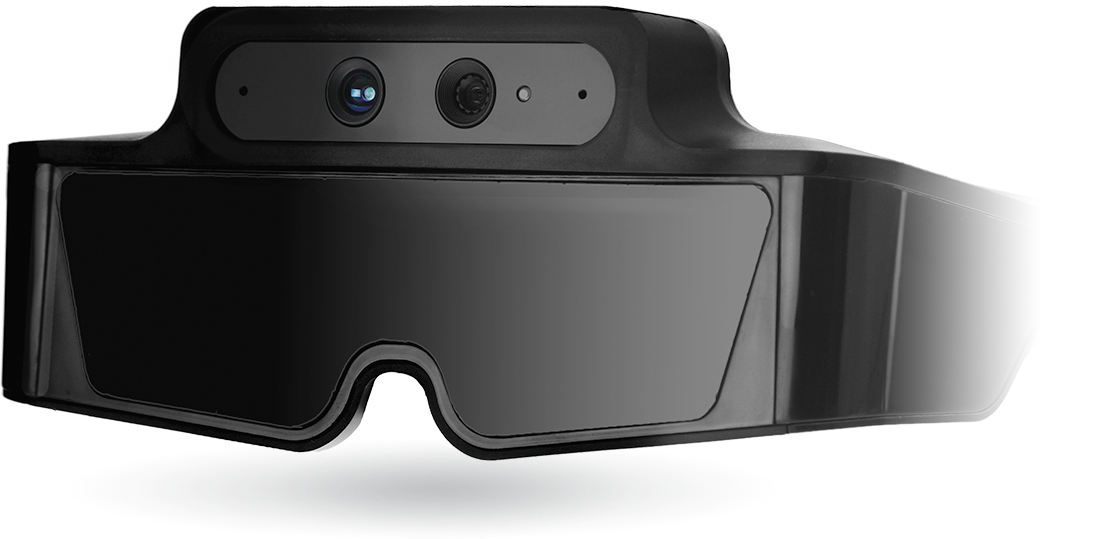
\includegraphics[width=\textwidth]{MetaOneGlasses}
            \caption{A pair of META One glasses.}
            \label{fig:metaone}
        \end{figure}
        
        The challenge with the META One was to get it working in Unity.
        There is a Meta SDK which allows for Unity games to work with
        the META One, but AR itself is still in development (as of
        writing this report), and the META One glasses are experimental
        at best. The SDK that we used first was also very buggy (due to the
        experimental nature of the META One). Also, the META One has a very
        limited field-of-view (the field-of-view was so limited that, during
        one of our first tests with our coach, the coach had to sit back
        to keep everything tracked, which, especially considering that they
        had to move markers as well as track the environment continuously,
        was less than ideal). However, the SLAM tracking built into the
        META allows for game objects to continue to be rendered on a marker
        even if the marker is outside of the view of the META. SLAM tracking
        is explained in subsection \ref{ssec:slamloc}.
        
        \subsection{SLAM tracking} \label{ssec:slamloc}
            SLAM is an acronym, which means Simultaneous Localization And
            Mapping. It stands for a computational problem making a map
            from an unknown environment while updating the location of the
            agent in the same environment. These problems cannot be solved
            independently from each other, as updating a map usually involves
            knowing the location of the agent before any accurate updates
            can be made, and vice versa. Several algorithms have been developed
            for solving this problem, and there is even a platform, called OpenSLAM,
            which contains several open source algorithms which solve this
            problem.
            
            However, the algorithms are beside the point. the real benefit of 
            using SLAM with AR is that SLAM tracking allows the META One to
            render the game objects belonging to a marker while keeping them
            rendered once the marker leaves the field-of-view of the META One.
            Considering that the field-of-view of the META One is not that large
            (As seen in our research report under Appendix \ref{app:researchreport}),
            this is a huge benefit. The META One also has built-in support for
            SLAM tracking of objects, which meant that no time had to be spent
            on developing algorithms.


    \section{Synchronization of World State} \label{sec:synchronization}
        Because the game is played by multiple people, the state of the world
        somehow has to be synchronized between all players. To do this, we 
        considered two major options:
        
        The first option was to use the built-in Network View component in 
        Unity. This would allow Unity to take care of most synchronization,
        which in turn could make implementing the synchronization particularly
        easy. However, due to the way the Meta One glasses manipulate the 
        positions and rotations of game objects to fit the orientation of the 
        player's head, synchronizing these positions would result in incorrect
        positions for other players. Instead, a custom serialization method 
        would have to be implemented to undo the manipulation by the Meta One
        and then apply the correct manipulation for each of the other players.

        Another option was to introduce a master server with camera that hosts
        the game, and provides raw positions and rotations of markers exactly as
        they were placed on the table. The only thing left to do would be to
        move and rotate the objects for each player to match that player's view
        of the playing area.

        We chose the second option for the following reasons:

        \begin{itemize}
            \item A master camera can see all markers at any one time, which
            means that there is never any uncertainty.
            \item The first option requires complex peer-to-peer synchronization
            and conflict resolution when multiple players see an overlapping set
            of markers.
            \item Unlike the cameras worn by players, the master camera is not
            constantly moving, meaning that marker recognition is not affected
            by motion blur.
        \end{itemize}
        
        Aside from the aforementioned reasons, we also made the decision to go
        with the second approach because it allowed us more control over the 
        internal workings of the network functionality and the marker tracking.
        See section \ref{sec:markerdetection} for the details about the marker
        detection performed by the server.

    \section{Marker Detection} \label{sec:markerdetection}
        The META One glasses come with marker detection built-in and we had
        difficulty replacing this detection with a custom system. That meant
        that our master camera server has to detect the same type of marker.
        Luckily the META markers have a very simple design. They're 6 by 6 bits
        encoded as black and white squares with a black border around them, as
        shown in figure \ref{fig:metaonemarker}.

        \begin{figure}[!ht]
            \centering
            
\includegraphics{MetaMarker}
            \caption{A marker that can be recognized by the Meta.}
            \label{fig:metaonemarker}
        \end{figure}

        These patterns map to an ID and are asymmetrical so that rotation can be
        resolved when they are detected. To easily find these markers on a table
        and board, we've also added a vibrant green border to them. This doesn't
        affect the META, but it makes segmentation of the markers from the
        background much more straightforward for the master camera. These final
        markers are shown in figure \ref{fig:finalmarker}.

        \begin{figure}[!ht]
            \centering
            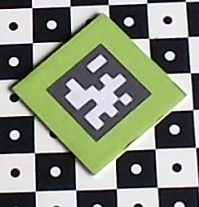
\includegraphics{FinalMarker}
            \caption{A marker that can be recognized by the Meta and the master camera.}
            \label{fig:finalmarker}
        \end{figure}

        The corners of the playing surface are set using red markers, as shown
        in figure \ref{fig:cornermarkers}. The need for these is explained in
        the next sections, which also describe the rest of the marker tracking
        process on the server.

        \begin{figure}[!ht]
            \centering
            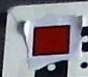
\includegraphics{CornerMarker}
            \caption{A marker that indicates a playing surface corner.}
            \label{fig:cornermarkers}
        \end{figure}

        \subsection{Board detection}
            The first step to tracking is to isolate the playing surface from
            the camera image and to apply perspective correction to it. The red
            corner markers described above are used to find the bounds of the
            rectangular playing surface. An example of the transformation is
            shown in \ref{fig:boarddetection}.

            \begin{figure}[!ht]
                \centering
                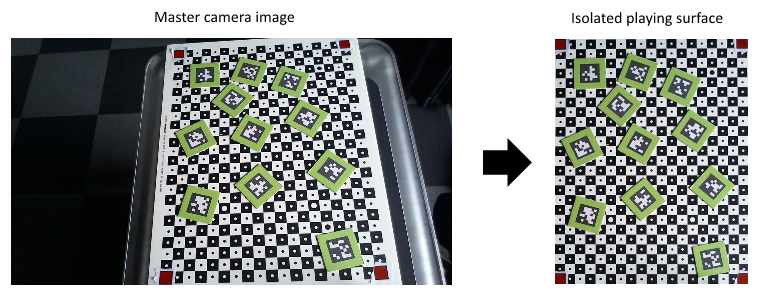
\includegraphics[width=\textwidth]{BoardDetection}
                \caption{Example of detecting playing surface and isolating it.}
                \label{fig:boarddetection}
            \end{figure}

            The four red corner markers are located by converting the input
            image to the HSV color space and thresholding on a red-like hue and
            a high saturation. The noise is then removed using a morphological
            open operation and the system verifies that 4 contours are found. If
            an amount of contours other than 4 is found, the user is prompted to
            move the camera such that the entire playing surface is visible and
            there are no other vibrant red objects in view.

            The corners of the playing surface are required to compute the
            transformation for the perspective correction. The perspective
            correction is required to recognize markers and their location
            correctly by making the camera view look like it views the board
            from above.

        \subsection{Marker detection}
            The markers are first segmented from the playing surface using their
            vibrant green borders, again through the HSV color space. The mask
            that results from this is cleaned up again using morphological open
            and close operations. An example of such a mask is shown in
            figure \ref{fig:markerthresholding}.

            \begin{figure}[!ht]
                \centering
                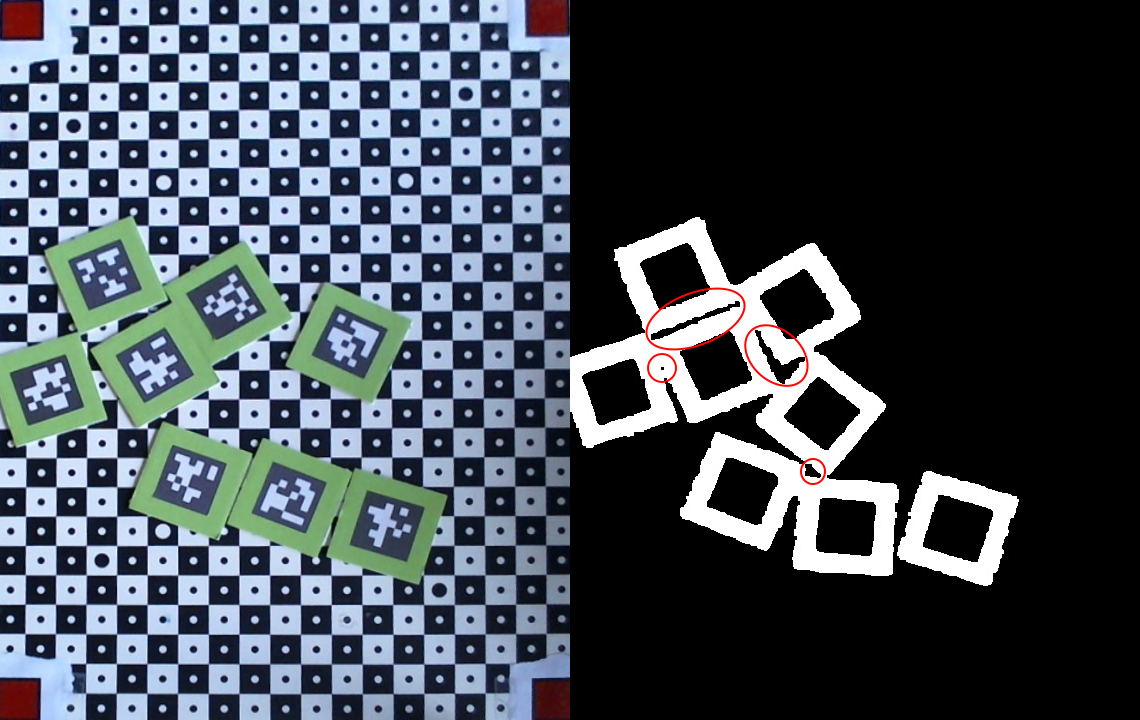
\includegraphics[width=\textwidth]{MarkerThresholding}
                \caption{Example of thresholding markers with false holes highlighted.}
                \label{fig:markerthresholding}
            \end{figure}

            It is evident from the example that finding the borders alone is not
            sufficient, because they will connect when the markers are close
            together. However, we know that each marker contains a non-green
            center with the actual code, which shows up as holes in the mask. We
            can detect these holes by using OpenCV's contour finding feature
            using hierarchy mode and selecting just the contours that lie
            directly within the outer contours.

            Unfortunately, when markers are really close together, some other
            holes appear as well (highlighted in the example). We remove these
            by filtering the contours using the following criteria:

            \begin{itemize}
                \item Holes have a minimum width and height of 8 (minimum
                required for reading a pattern)
                \item Holes are square to within a tolerance of 15\%
                \item Holes have the same size as the median size of all
                detected holes to within a tolerance of 15\%
            \end{itemize}

            Especially the last one works very well for a playing surface with
            many markers, where the signal to noise ratio is high. The process
            finished by returning the contours of all the holes detected as
            markers.

        \subsection{Marker recognition}
            The marker recognition process takes the contours from the marker
            detector stage. It starts by finding the minimum area bounding
            rectangle around a contour to find its rotation. The source image is
            then rotated to straighten the marker.

            The next step is to isolate the pattern from the marker. It first
            converts the image to grayscale and resizes it to 8 by 8 pixels (the
            6 by 6 pattern with the 1 pixel wide border within the marker). The
            average brightness across the pattern is found and used to threshold
            the black and white pixels. The image is then cropped to just the 6
            by 6 pixel pattern. The original scale of the marker is also stored
            to later scale the marker positions.

            The final step is to identify which known pattern the detected
            pattern best matches. Although the marker has already been
            straightened, it could still be rotated by 90, 180 or 270 degrees.
            For that reason, the system searches all known patterns using the
            four possible rotations of the input. It determines the best match
            using the Hamming distance between 2 patterns. The detected best
            matching rotation is then added to the rotation needed to straighten
            it to compute the complete rotation.

            The marker recognition system does not verify if the best pattern
            match is good enough, it will happily return a best match with
            confidence score \verb#0.0#.

        \subsection{Marker tracking}
            The marker tracker system takes the output from the marker detection
            and recognition stages (position and match) from each frame and uses
            this data to track the movement of markers across frames. It
            primarily does this by checking which marker position from the
            previous frame each new marker position is closest to. It uses the
            pattern matching results only when a marker is not moving quickly.
            It uses results from multiple frames to smoothen positions and
            rotations using a moving average that is discarded when a marker
            has sudden changes. It also detects if a marker has been removed by
            measuring if it hasn't been seen for a long while.

            All of the changes it detects, like new markers, moved markers and
            removed markers are added to a list each frame and returned to the
            main application. The main application then broadcasts these changes
            over the server socket to the META One clients.
        
    \section{Networking and the OpenCV server} \label{sec:network}
        The game depends on a server application with a master camera. The 
        server application detects the position and rotation of markers in the 
        playing area. It does this through the use of a central so-called master 
        camera, that is position so that the entire playing area is visible from 
        the camera.
        
        The server application is written in C++ and is based on OpenCV and the 
        Qt framework. We decided to implement the server outside of Unity, since 
        Unity does much more than what we need of the server. The server only 
        acts as a way to track all markers even if they aren't seen by any of 
        the players, and to facilitate synchronizing state changes with all 
        players. For example, if a remote player rotates an object in the game, 
        the details about that rotation is sent to the server, which then 
        distributes it to all other players.
        
        A more detailed description about the communication between the Unity 
        clients and the server can be found in paragraph \ref{ssec:communication}.
        The use of the master camera to detect markers is described in paragraph
        \ref{ssec:mastercamera}.
                
        \subsection{Communication between C\# and C++} \label{ssec:communication}
            Communication between the Unity clients and the OpenCV server 
            happens through the use of sockets. For the Unity side, the Socket 
            facility built into the C\# runtime is used. For the OpenCV server, 
            the TCP Socket facility of the Qt Network module is used for 
            providing a server socket capable of handling multiple clients. 
            
            The protocol used for communication is kept very simple to reduce 
            network load and for simplicity. The protocol consists of a number
            tag indicating the message type followed by the actual message 
            content. To facilitate the features the game provides, the following
            message types are used:
            
            \begin{description}
                \item[Position Update] Sent by the server whenever it detects a 
                                       change in a marker position.
                \item[Position Delete] Sent by the server whenever a marker is
                                       removed from the playing field.
                \item[Rotation Update] Sent by remote players to indicate they 
                                       have rotated an object. This message is 
                                       forwarded to all connected clients by the
                                       server.
                \item[Ping Message]    Sent by the server and clients to indicate 
                                       they are still connected and listening.
            \end{description}
        
        \subsection{The master camera} \label{ssec:mastercamera}
            ...
            
    \section{Distinguishable markers} \label{sec:markers}
        ...